\raggedright
\section{Profiling}

texto
\newline

\subsection{Education}
Variable Type: Categorical Nominal.\newline
Recall: the Education variable describes the level of studies the consumer has (2nd cycle, Basic, Graduation, Master, PhD).

\begin{figure}[H]
    \centering
    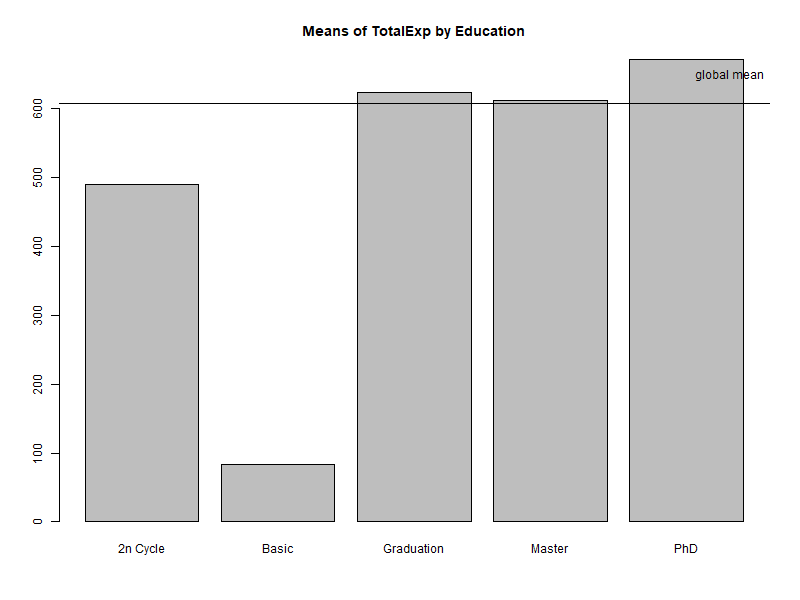
\includegraphics[width=0.8\linewidth]{Imatges/mean_barplot_TotalExp.png}
    \caption{Descripció}
    \label{fig:scree_plot}
\end{figure}
\newline
With a mean barplot we can see the total expent depending on the level of studies, where it is evident that the basic education group spends much less money on their purchase.

\begin{figure}[H]
    \centering
    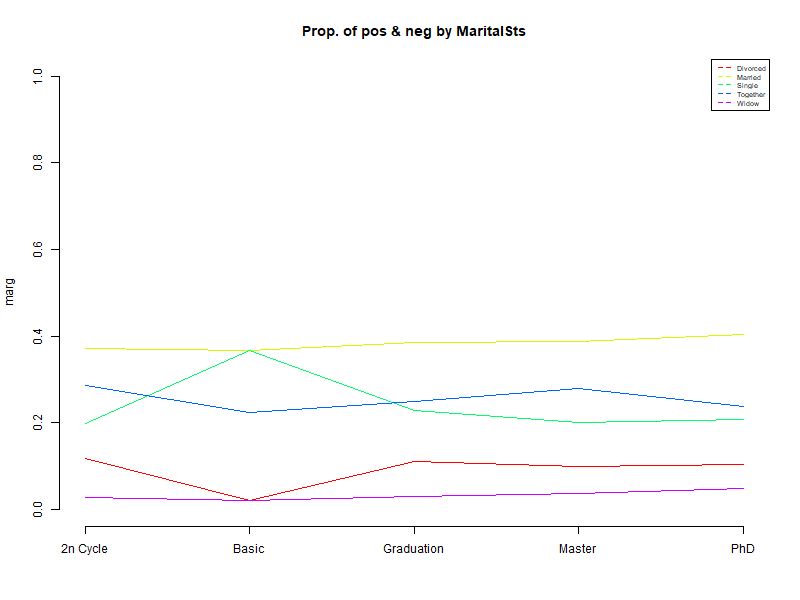
\includegraphics[width=0.8\linewidth]{Imatges/prop_cond_class_MaritalSts_4_legend.png}
    \caption{Descripció}
    \label{fig:scree_plot}
\end{figure}
\newline
Comparing with the marital status we can see that independently of their studies, the customers usualy are married or together. It is worth noting that those with a basic education level are more often married or single.
\begin{figure}[H]
    \centering
    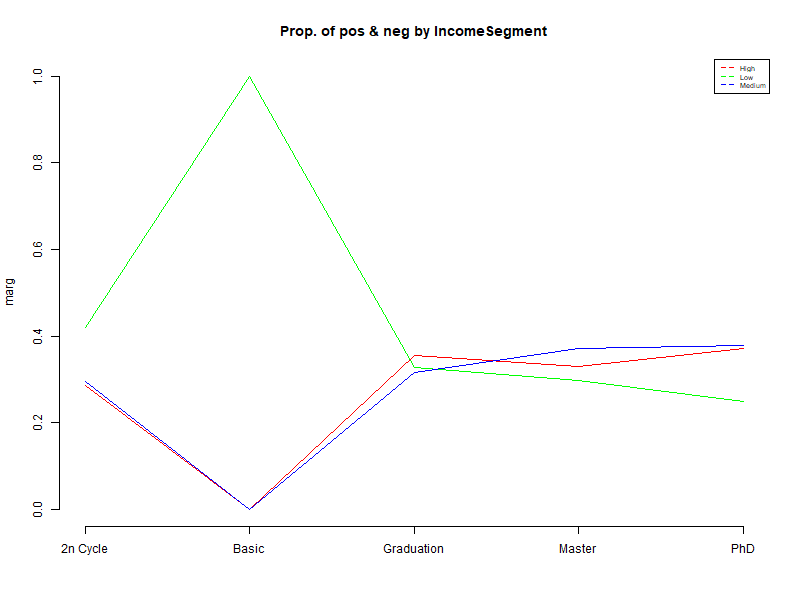
\includegraphics[width=0.8\linewidth]{Imatges/prop_cond_class_IncomeSegment_4_legend.png}
    \caption{Descripció}
    \label{fig:scree_plot}
\end{figure}
\newline
Comparing the income segment we can see that the basic level has the highest frequency with low segment. It shows that they are the ones with the lowest incomes, followed by those with a second-level education, and that there is not much difference among the rest.
\begin{figure}[H]
    \centering
    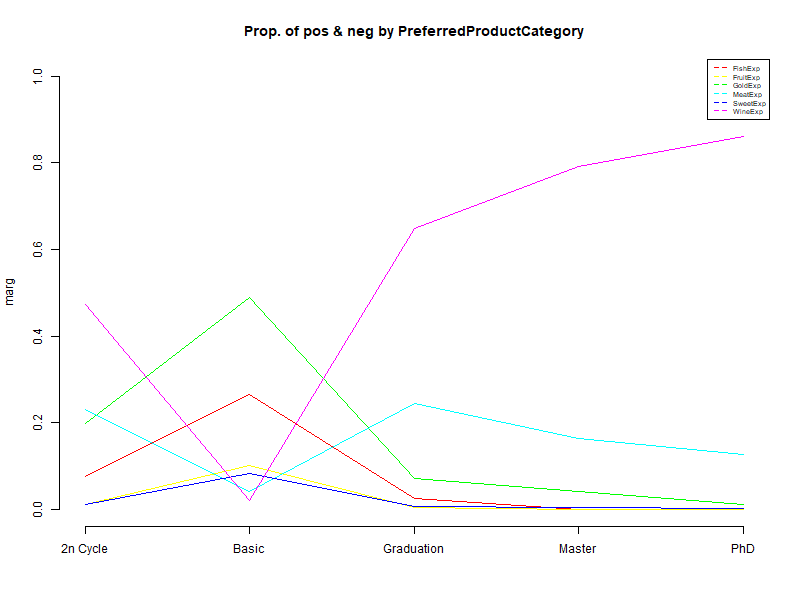
\includegraphics[width=0.8\linewidth]{Imatges/prop_cond_class_PreferredProductCategory_4_legend.png}
    \caption{Descripció}
    \label{fig:scree_plot}
\end{figure}
\newline
About their most purchased product category, we can see that as the level of education increases, there is a tendency to spend more on wine, the customers with lower education levels prefer to buy gold, and those with a graduation level education tend to spend on meat.

\subsection{MaritalSts}
Variable Type: Categorical Nominal.\newline
Recall: the MaritalSts variable describes the marital status of the customer (Divorced, Married, Single, Together, Widow).

\begin{figure}[H]
    \centering
    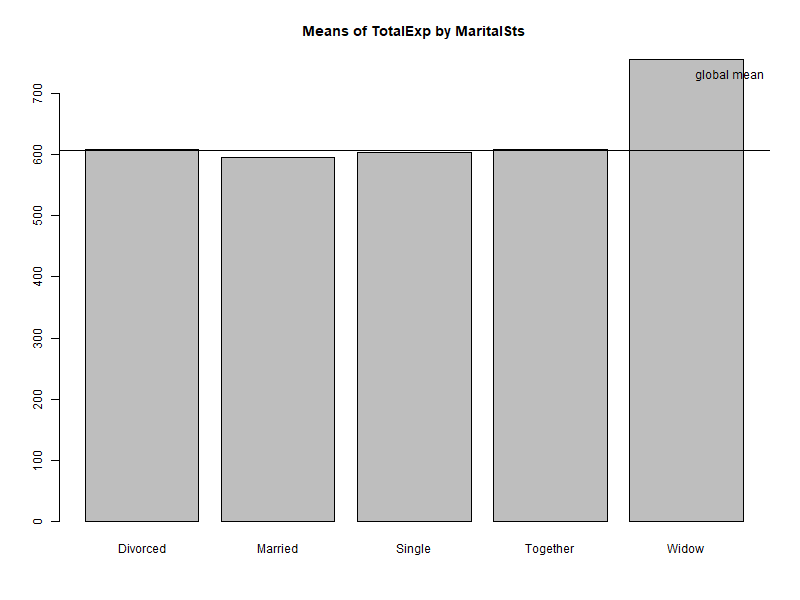
\includegraphics[width=0.8\linewidth]{Imatges/mean_barplot_TotalExp(2).png}
    \caption{Descripció}
    \label{fig:scree_plot}
\end{figure}
\newline
With a mean barplot we can see that the total expenditure by marital status is quite uniform, despite widow customers that spends more on average.

\begin{figure}[H]
    \centering
    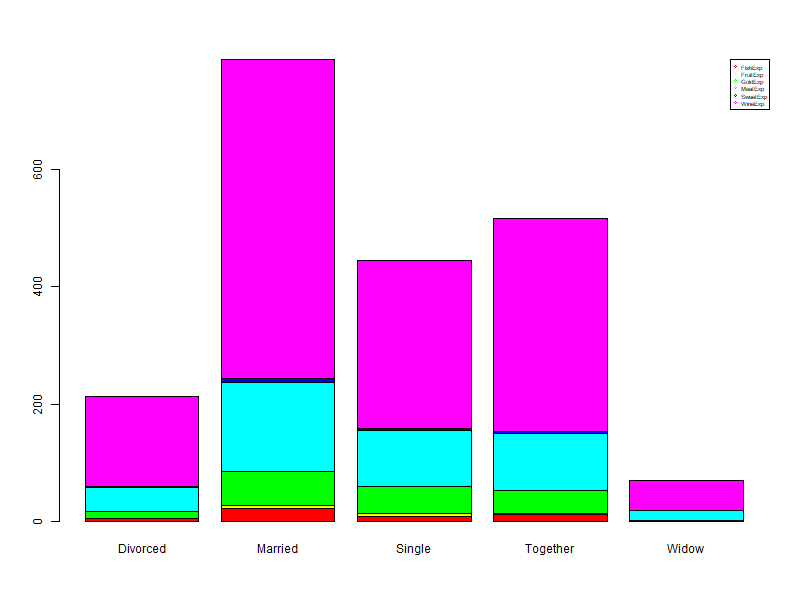
\includegraphics[width=0.8\linewidth]{Imatges/stacked_barplot_counts_PreferredProductCategory_10_legend.png}
    \caption{Descripció}
    \label{fig:scree_plot}
\end{figure}
\newline
It is interesting to observe that regardless of marital status, the main product is wine, followed by meat.

\subsection{IncomeSegment}
Variable Type: Numerical Discrete.\newline
Recall: ...

\begin{figure}[H]
    \centering
    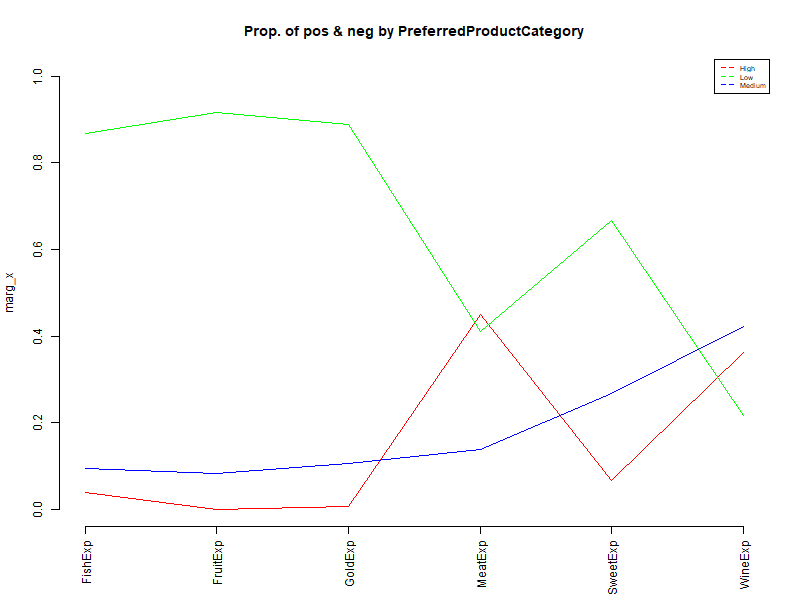
\includegraphics[width=0.8\linewidth]{Imatges/prop_cond_col_var_x_PreferredProductCategory_8_legend.png}
    \caption{Descripció}
    \label{fig:scree_plot}
\end{figure}
\newline
With this graph, it can be observed that the preferred category of customers varies depending on their segment. This shows how different their main interests are when it comes to spending their income.

\subsection{HasChildren}
Variable Type: Categorical Binary.\newline
Recall: the HasChildren variable  whether the customer has children or not (0 or 1).
Variable Type: Numerical Discrete.\newline

\begin{figure}[H]
    \centering
    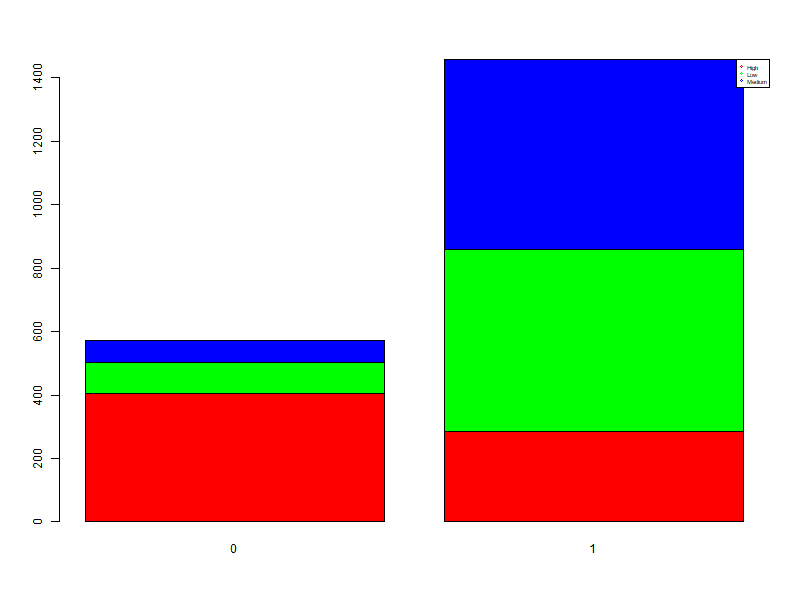
\includegraphics[width=0.8\linewidth]{Imatges/stacked_barplot_counts_IncomeSegment_10_legend.png}
    \caption{Descripció}
    \label{fig:scree_plot}
\end{figure}
\newline
In this graph, we can see that our sample has more consumers with children than without them, and the most consumers with children have a medium or low income status. On the other hand, those without children have a higher status.
\begin{figure}[H]
    \centering
    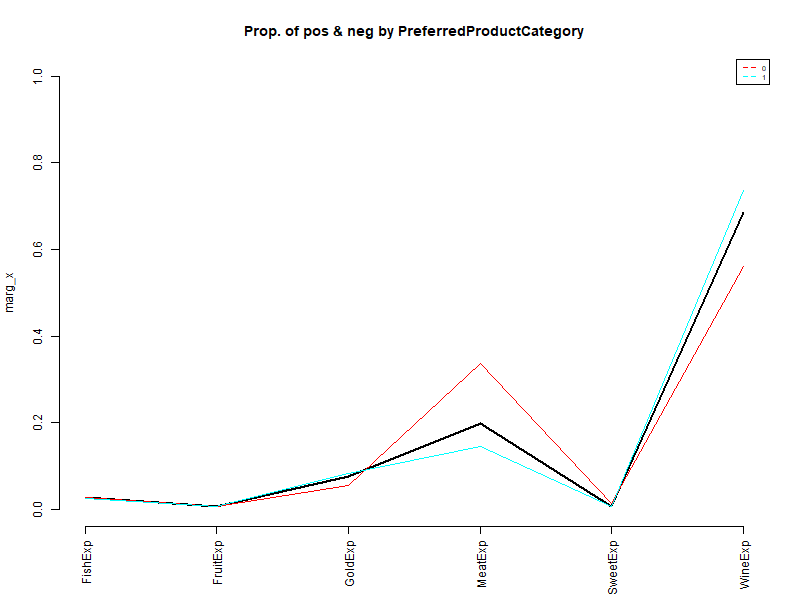
\includegraphics[width=0.8\linewidth]{Imatges/prop_cond_class_var_x_PreferredProductCategory_6_legend.png}
    \caption{Description }
    \label{fig:scree_plot}
\end{figure}
\newline
Regardless of whether they have children or not, the preferred category does not vary among consumers.


\subsection{PrefereredChannel}
Variable Type: Categorical Nominal.\newline
Recall: the PrefereredChannel variable describes the channel with highest frequency.

\begin{figure}[H]
    \centering
    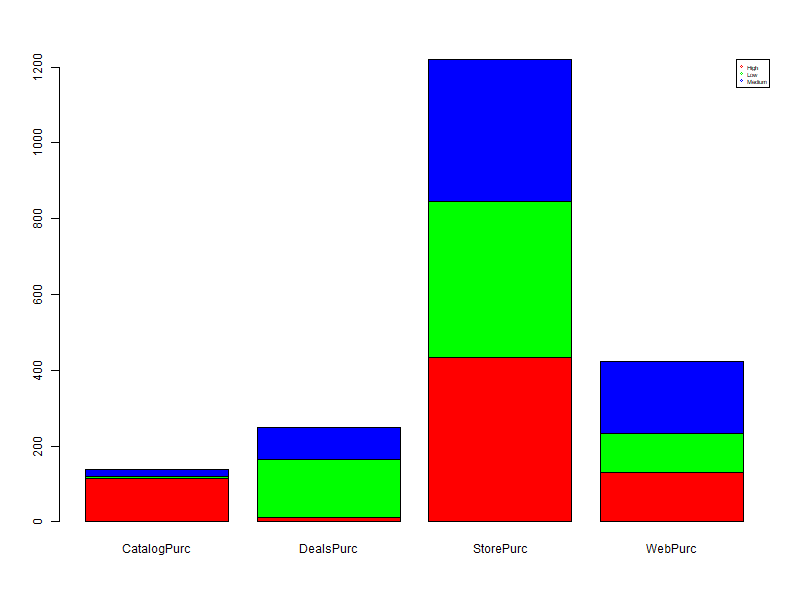
\includegraphics[width=0.8\linewidth]{Imatges/stacked_barplot_counts_IncomeSegment_10_legend(channel).png}
    \caption{Description }
    \label{fig:scree_plot}
\end{figure}
\newline
In this graph, we can observe the relationships between the preferred channel and income status. It can be seen that the vast majority prefer to shop in-store. However, it is worth noting that those with a medium status mainly shop online, those with a high status mainly shop via catalog, and those with a low status mainly shop based on promotions.


\subsection{PrefereredProductCategory}
Variable Type: Categorical Nominal.\newline
Recall: the PrefereredProductCategory variable describes the channel with highest frequency.
\begin{figure}[H]
    \centering
    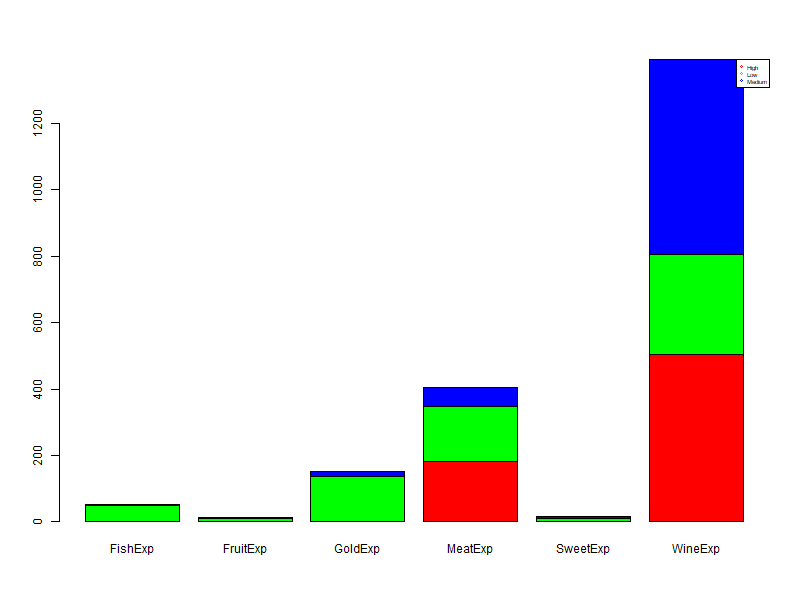
\includegraphics[width=0.8\linewidth]{Imatges/stacked_barplot_counts_IncomeSegment_10_legend(category).png}
    \caption{Description }
    \label{fig:scree_plot}
\end{figure}
\newline
Surprisingly, regardless of income status, the most preferred category is wine (although there is a much bigger difference between high and medium status compared to low). It is also important to note that the other less preferred categories are usually dominated by the low-income group.
